\chapter{Clustering by atomic bonds}
The aim of the simple structure evaluation is to discourage ASLA from choosing isolated atoms disconnected from the template structure, since these choices are not as stable as a single, coherent molecule. In order to solve this problem, the local feature vector of an atom will be a vector of integers, representing the number and type of atoms it is bonded to. Each composition of bonds corresponds to a cluster, which means that the bonds of an atom describes the cluster it belongs to. \\

The goal is to see this method of clustering, where the number and type of bonds of each atom determines its local energy, work and improve the performance of ASLA on this $C_6H_6$-structure search. Provided that it does, the aim would then be to design a more 'unbiased' local feature vector that doesn't directly determine what a good structure is and what is not. These local features would then be grouped using a clustering algorithm as described in chapter 3.


\section{Structure representation}

\begin{figure}
	\centering
	\centerline{
		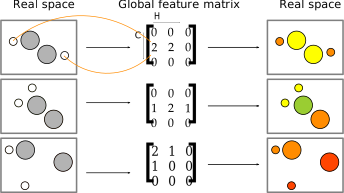
\includegraphics[width=\columnwidth]{graphics/structure_representation.pdf}
		}
	\captionsetup{width=1.2\columnwidth}
	\caption{Visualization of how structures are represented in a feature matrix. For illustration purposes the structures only consist of $C_2H_2$. Each entry in the matrix corresponds to the number of atoms with some specific bonds. As an example with the top structure shown, both $H$-atoms have $1$ $C$ bond an $0$ $H$ bonds, which is shown in the matrix at row 2 column 1. After examining all atoms in the structure, the matrix is flattened into a vector to estimate the local energy of each cluster. The structures can then be colored by the total number of bonds of each atom.}
	\label{fig:struc_representation}
\end{figure}
% Udregning af clusters
Each complete structure is analyzed using a feature function $g$, which for each atom in the structure will count all neighboring atoms within a $\SI{1.60}{\AA}$ radius, which is then considered a bond between the two. Thus the local feature vector becomes 
\begin{equation}
	\mathbf{f}_i = g(\mathbf{s}^{(I)}_{final}) =
	\begin{bmatrix}
	n_C^{(i)} \\
	n_H^{(i)}
	\end{bmatrix}.
\end{equation}
Here $i$ is the atomic index, $\mathbf{s}^{(I)}_{final}$ being the complete grid of structure $I$ and $n$ being the number of bonded atoms of type $C$ or $H$.

The reason that the bonding range is $\SI{1.60}{\AA}$ is that in the global energy minimum structure built with $C_6H_6$, benzene, the distance between some of the neighboring $C$-atoms on the grid is $\sqrt{10}/2 \, \SIUnitSymbolAngstrom \approx \SI{1.58}{\AA}$. All of these bonds should be found when analyzing the structure to give an accurate representation of why the structures is so stable. This means that all $C$-atoms will have the same number of bonds and likewise for the $H$-atoms in the structure. This would not be the case for a lower bonding range of e.g. $\SI{1.5}{\AA}$, which would not represent benzene as a very stable structure to build.\\

The number and type of neighbors of one atom will be represented by a list of integers, one for each atom type in the structure. This list of integers is the coordinate of an entry in a tensor with dimensions $N_t + 1$, with $N_t$ being the number of atoms of type $t$ in the structure (e.g. for $C_2H_2$ it is a $3\times3$-matrix as seen in figure \ref{fig:struc_representation}). Each entry in the tensor counts the number of atoms in the structure that match their coordinates, with each entry counting as a seperate cluster. The tensor is then flattened to create the global feature vector $\mathbf{F}$ of that structure. When building $C_{N_C}H_{N_H}$-structures we get the following representation of the structure

\begin{align}
\mathbf{F}_I(\mathbf{f}_1,...,\mathbf{f}_N) &= 
\begin{bmatrix}
n_{0,0} 				& \cdots & n_{0, \, (N_H + 1)} \\
\vdots 					& \ddots & \vdots \\
n_{(N_C + 1) \, , 0} 	& \cdots & n_{(N_C + 1)  \, , (N_H +1)}
\end{bmatrix}
\sim
\begin{bmatrix}
n_{00} \\
n_{01} \\
\vdots \\
n_{N_H N_C}
\end{bmatrix} 
\end{align}

%% Farvelægning af atomer
Atoms are colorized according to the total number of bonds. The colorscheme for each number of bonds is: 0 - Red, 1 - Orange, 2 - Yellow, 3 - Yellowgreen, 4 - Limegreen. No structures with 5 or more bonds are depicted in this project, but the color is set to be darker shades of green for each bond above 4. Atom coloring is depicted figure \ref{fig:struc_representation}. 

\section{Results}
\begin{figure}
	\centering
	\centerline{
		
\includegraphics[width=1.4\columnwidth]{graphics/bonding_demo.pdf}
	} % Centerline centrerer brede figurer
	\captionsetup{width=1.2\columnwidth}
	\caption{Demonstration of local features for each atom of a completed structure. 
		\textbf{Frame 1:} The red $H$-atom is too far away from the rest of the structure and is considered isolated by the feature function $g$. 
		\textbf{Frame 2:} Moving the $H$-atom to the right will bring it close enough to the remaining structure for $g$ to consider it a bond.
		\textbf{Frame 3-4:} Further moving the atom to the right will also change the representation (color) of the other atoms as they become bonded or bonds break with this atom. Note in frame 3 that this representation only has a maximum distance and so it doesn't penalize placing atoms too close to each other.}
	\label{fig:bonding_demo}
\end{figure}



%% Forudsigelse af energi isoleret fra ASLA
%% Forudsigelse figur
\begin{figure}
	\centering
	\centerline{
		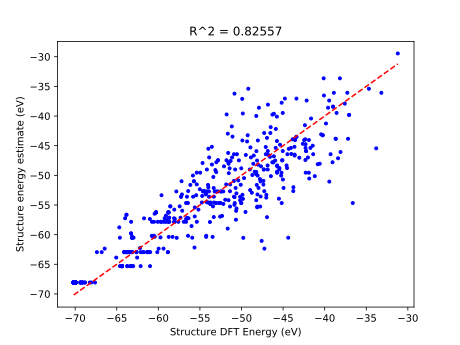
\includegraphics[width=\columnwidth]{graphics/energy_prediction.pdf}
		}
	\captionsetup{width=1.2\columnwidth}
	\caption{Demonstration of how estimating the potential energy of structures built by ASLA can be done using local energies dependent on the number and type of bonds of each atom in the structure. The $500$ blue points come from a random sample of builds by an agent that found the global energy minimum of $\SI{-70.17}{\electronvolt}$. These structures have all had their potential energy estimated by a DFT calculation, which is their position on the first axis. Their position on the second axis is determined by their estimated energy. The red line indicates the points where the DFT energy and the estimate are equal.}
	\label{fig:energy_prediction}
\end{figure}

Using the demonstrated ability to count the bonds of each atom, it is then tested if it is possible to predict the energy of completed structeres by clustering local energies according to bonds as in equation \eqref{eq:Matrix_problem_rewritten}. Each entry in the global feature vector $\mathbf{F}_I$ from equation \eqref{eq:Energy_bundles_matrix} represents the number of atoms with a specific number and type of neighbours in structure $I$.\\ 

As can be seen on figure \ref{fig:energy_prediction} this method of using ridge regression to estimate the local energy of each bond-environment can successfully estimate the approximate energy of $C_6H_6$-structures built by ASLA. By calculating the features of $500$ random structures from an agent that found the global minimum, an estimate for the local energies of the different bond-enviroments $\bm{\varepsilon}$ was calculated. Using these energies, the energy of another $500$ random structures were calculated. \\

%% Hvor mange overlever mit filter ud af N?
%% Frasorterings figur
\begin{figure}
	\centering
	\centerline{
		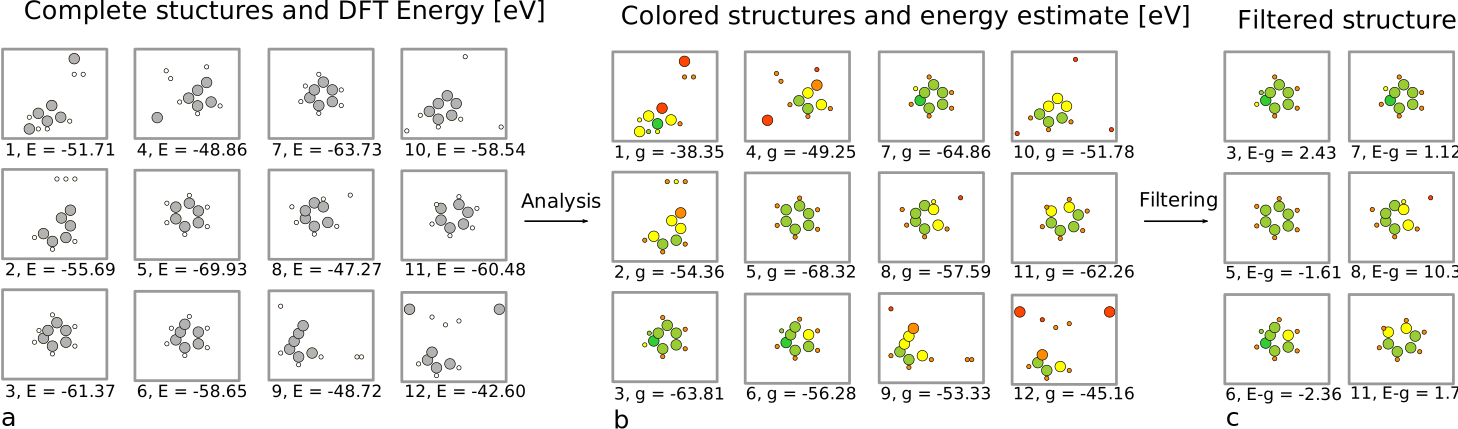
\includegraphics[width=1.4\columnwidth]{graphics/filtering_demo.pdf}
		}
	\captionsetup{width=1.4\columnwidth}
	\caption{Demonstration of how the proposed filtering algorithm works. The estimated energy of each cluster is calculated from $500$ structures. \textbf{a:} The agent builds $N$ structures that are saved in a list. In this example the DFT calculation has been done to show the true target property of each structure. \textbf{b:} A feature vector is then calculated for each structure and using this, the energy of the complete structure is estimated. \textbf{c:} The filtering then consists of choosing the $N/2$ structures with the lowest estimated energy.}
	\label{fig:filtering}
\end{figure}

Using this method to estimate the energy of builds, it is then attempted to implement an algorithm that can choose e. g. the $50\%$ best structures from a list. An illustration of this algorithm can be seen on figure \ref{fig:filtering}. An enlarged version can be seen on figure \ref{fig:App_Filtering} in the appendix. \\

Using a number of complete structures and their calculated DFT energies, the energies of the different bond-clusters is calculated. Then, the agent is asked to build $N$ structures, making no expensive DFT calculation for any of them. The energy of each structure is then predicted, estimated from the found bonds of each atom in the structure. The structures are then sorted from lowest(most stable) to highest(least stable) with respect to their estimated potential energy. Some percentage of the structures with lowest energy are then kept. One structure is then chosen randomly among the remaining structures as the one to have a DFT energy calculation done. This chosen structure will likewise have all building steps and final structure saved in the replay buffer for training in future episodes. \\

To demonstrate the ability of the filter to remove structures with isolated atoms, 5 different estimates to $\bm{\varepsilon}$ were made. Each had the features from 500 structures made from an agent that had found the global minimum. Each of these $\bm{\varepsilon}$ then predicted the energy of $N=50$ random structures also made by the agent and recorded the number of structures containing isolated atoms, $n_{pre}$. After filtering, keeping only the 25 structures with lowest potential energy, the number of structures containing isolated atoms, $n_post$, was recorded. The relative change $(n_{post}-n_{pre})/n_{pre}$ is then calculated for the run, and each run is repeated 10 times. In total, for 5 different $\bm{\varepsilon}$ each make 10 runs, in each run building 50 structures and choosing the best 25. This resulted in a relative reduction of isolated structures of $\SI{72.3 \pm 5.8}{\percent}$. On average, almost $3/4$ of the structures with isolated atoms are removed by filtering using this method!




